%------------------------------------------------------------------------------
% Template file for the submission of papers to IUCr journals in LaTeX2e
% using the iucr document class
% Copyright 1999-2013 International Union of Crystallography
% Version 1.6 (28 March 2013)
%------------------------------------------------------------------------------

\documentclass[preprint]{iucr}              % DO NOT DELETE THIS LINE

     %-------------------------------------------------------------------------
     % Information about journal to which submitted
     %-------------------------------------------------------------------------
     \journalcode{J}              % Indicate the journal to which submitted
                                  %   A - Acta Crystallographica Section A
                                  %   B - Acta Crystallographica Section B
                                  %   C - Acta Crystallographica Section C
                                  %   D - Acta Crystallographica Section D
                                  %   E - Acta Crystallographica Section E
                                  %   F - Acta Crystallographica Section F
                                  %   J - Journal of Applied Crystallography
                                  %   M - IUCrJ
                                  %   S - Journal of Synchrotron Radiation
\usepackage{graphicx}
\usepackage[T1]{fontenc}
\usepackage[utf8]{inputenc}
\usepackage{amsmath}

\begin{document}                  % DO NOT DELETE THIS LINE

     %-------------------------------------------------------------------------
     % The introductory (header) part of the paper
     %-------------------------------------------------------------------------

     % The title of the paper. Use \shorttitle to indicate an abbreviated title
     % for use in running heads (you will need to uncomment it).

\title{Application of signal separation to diffraction image compression and serial crystallograpby}
%\shorttitle{Short Title}

     % Authors' names and addresses. Use \cauthor for the main (contact) author.
     % Use \author for all other authors. Use \aff for authors' affiliations.
     % Use lower-case letters in square brackets to link authors to their
     % affiliations; if there is only one affiliation address, remove the [a].

\cauthor[a]{Jérôme}{Kieffer}{jerome.kieffer@esrf.fr}
\author[b]{Forename}{Surname}
Nicolas Coquelle
Jonathan P. Wright
Gavin Vaughan
Jianluca santoni
daniele de sanctis

\aff[a]{European Synchrotron Radiation Facility;71, avenue des Martyrs;CS 40220;38043 Grenoble Cedex 9 \country{France}}
\aff[b]{Second affiliation address}

     % Use \shortauthor to indicate an abbreviated author list for use in
     % running heads (you will need to uncomment it).

%\shortauthor{Soape, Author and Doe}

     % Use \vita if required to give biographical details (for authors of
     % invited review papers only). Uncomment it.

%\vita{Author's biography}

     % Keywords (required for Journal of Synchrotron Radiation only)
     % Use the \keyword macro for each word or phrase, e.g. 
     % \keyword{X-ray diffraction}\keyword{muscle}

%\keyword{keyword}

     % PDB and NDB reference codes for structures referenced in the article and
     % deposited with the Protein Data Bank and Nucleic Acids Database (Acta
     % Crystallographica Section D). Repeat for each separate structure e.g
     % \PDBref[dethiobiotin synthetase]{1byi} \NDBref[d(G$_4$CGC$_4$)]{ad0002}

%\PDBref[optional name]{refcode}
%\NDBref[optional name]{refcode}

\maketitle                        % DO NOT DELETE THIS LINE

\begin{synopsis}
Precise background assessement and application to single crystal image compression and serial crystallography data preprocessing. 
\end{synopsis}

\begin{abstract}
Abstract goes here.
\end{abstract}


     %-------------------------------------------------------------------------
     % The main body of the paper
     %-------------------------------------------------------------------------
     % Now enter the text of the document in multiple \section's, \subsection's
     % and \subsubsection's as required.

\section{Introduction}

%\cite{Cheetah2014}
The Synchrotron serial crystallography beamline (ID29 at ESRF) has been built to \ldots
In this setup samples will be carried in front of the beam and a Jungfrau 4M detector records 


\section{Algorithm for the separation of amorphous background from Bragg peaks}
\subsection{Background scattering}
The core idea of the separation of Bragg peaks from background is to consider that the background scattering 
is originating from unordered matter which gives some isotropic signal, preferably with smooth variations.
For this the raw signal has to be corrected from dark noise and any systematic anisotropic effects like polarization corrections.

The initial implementation in pyFAI \cite{pdj2013} relied on a 2D radial transform followed by a median filter in the azimuthal dimension 
to separate amorphous scattering from crystalline scattering.
Despite this method has been successfully used for large dataset analysis \cite{brocades}, it has several major drawbacks:
* The 2D averaging mixes the signal of several pixels and blures the signal. 
* Pixel-splitting is needed to leverage the moiré effect in the 2D averaging, but this increases further the blurring. 
* The filtered 1D curve obtained after the median shows sharp jumps from one azimuthal bin to its neighbor.
* Median filter is complicated and requires a lot of memory.
    
The coming sections present an efficient way to perform the azimuthal averaging and the associated variance propagation, 
and how it can be used to perform the statistical analysis to extract the background from a diffraction image. 

\subsection{Efficient azimuthal averaging and uncertainties evaluation}

\subsubsection{Preprocessing} is a pixel-wise correction for flat and normalization \cite{pyfai_2020}: 
\begin{equation}
I_{cor} = \frac{signal}{normalization}  = \frac{I_{raw} - I_{dark}}{F \cdot
\Omega \cdot P \cdot A \cdot I_0} 
\end{equation}

where $I_{raw}$ is the detector's raw signal, $I_{dark}$ is the dark current
image (it may also be the background image for certain experiments), $F$ is a 
factor accounting for the flat-field correction, $\Omega$ is the solid
angle subtended by a given pixel, $P$ is the polarisation correction term and
$A$ represents the detector's apparent efficiency due to the incidence angle of the
photon on the detector (for integrating detectors, high energy photons with
larger incidence angle see larger sensor thickness, and thus have higher
detection probability).
$I_{raw}$ may be normalized by the incoming flux $I_0$, which is
independent of the pixel position.

\subsubsection{Azimuthal averaging} was initially implemented using histograms but this was pretty slow.
Since the the geometry of the experimental setup is fixed during the acquisition, 
a look-up table listing all pixels contributing to every azimuthal bin can be built and used to speed-up calculations.
\begin{equation}
<I>_{r} = \frac{\sum\limits_{i \in bin_r} c_i \cdot signal_i}
                        {\sum\limits_{i \in bin_r} c_i \cdot normalization_i} 
\end{equation}

The azimuthal transformation can then be seen as a linear tranformation and implemented as a ``sparse-matrix times dense vector'' multiplication 
where the dense vector is simply the flattened view of the diffraction image\cite{pyFAI_gpu}. 
The CSR-sparse matrix representation is often used since it is very efficient to perform dot products with dense vectors.
In the case where pixel splitting is deactivated (i.e. each pixel contribute to a single bin) the numerical values in the sparse value ($c_i$) are always `one` (and zero elsewhere).
The sparse matrix multiplication can be used to sum efficiently values for all pixels belonging to the same bin.
To obtain the average value for a given bin, the summed signal must be divided by the summed normalization 
  
\subsubsection{Uncertainty evaluation from Poisson law.}
Photon counting suffered from several uncertainies, among which the most important one is usually the counting statistics (often refered as Poisson law)
stating that the variance for a pixel is at least the number of events counted.
Other sources of noise superimposes quadratically to the Poisson noise, like the dark-current noise:     

\begin{equation}
var(I) = (\sigma(I))^{2} = I_{raw} + (\sigma_{dark})^{2}  
\end{equation}

During the regrouping part, the coeficients of the sparse matrix needs to be squarred for the variance part as described: 
\begin{equation}
(\sigma_{r}(I))^2 = \frac{\sum\limits_{i \in bin_r} c_i^2 \cdot variance_i}
                  {\sum\limits_{i \in bin_r} c_i \cdot normalization_i} 
\end{equation}

One should distinguish the \textit{uncertainty of the mean} (sometimes referred are standard error of the mean, $sem$) 
which describes the precision with which the mean is known (and is described in \cite{pyfai_2020}),
from the \textit{uncertainty of the pixel value} (often referred are standard deviation, $std$). 
Those two value differ only the normalization: $sem = std/\sqrt(normalization)$.
Thus, the more data point, the more precisely is known the mean value.
Since this document focuses on pixel values and the precision of individual pixel values, the \textit{standard deviation} will systematically be used in this document.  

\subsubsection{Uncertainty evaluation from variance in a bin.}
If all pixels falling into a single bin should have the same numerical value and the deviation to this value can be seen as an estimation for the uncertainty.
This is far from being the case with single crystal diffraction images but can be assumed with pure background images.
Variance and standard deviation are usually obtained in two steps: one pass to calculate the average value and a second to calculate the deviation to the average. 
This double pass approach is very stable numerically and can be implemented using sparse matrix multiplication but requires the access of each pixel twice. 
 
Single pass implementation of variance are faster and offer the ability to perform parallel reductions, i.e. work with blocks of pixels.
\citeasnoun{variance2018} presents a complete review, with some key equations reported and adapted to the formalism of crystallography hereafter.
For example the weight for a pixel is $\omega_i = c_i \cdot normalization_i$
If $P$ is a partition of the ensemble of pixels falling into a given azimuthal bin, let $\Omega_{P}$, $V_{P}$ and $VV_{P}$  
be the weight sum, the weighted sum of $V$ and the weighted sum of deviation squared over the partition $P$: 
\begin{equation}
\Omega_{P} = \sum\limits_{i \in P} $\omega_i = \sum\limits_{i \in P} c_i \cdot normalization_i 
\end{equation}
\begin{equation}
V_{P} = \sum\limits_{i \in P} \omega_i \cdot v_i =  \sum\limits_{i \in P} c_i \cdot signal_i
\end{equation}
\begin{equation}
VV_{p} = \sum\limits_{i \in P} \omega_i \cdot (v_i - V_{P}/\Omega_{P})^2 
\end{equation}

The average and the variance are then expressed as:
\begin{equation}
<I>_P = V_{P}/\Omega_{P} =  
\end{equation}

\begin{equation}
(\sigma_P(I))^2 = VV_{P}/\Omega_{P} 
\end{equation}

Performing the union of two partition $A$ and $B$ allows the parallel reduction, which is especially efficient on GPU:
\begin{equation}
\Omega_{A \cup B} =  \Omega_{A} + \Omega_{B} 
\end{equation}

\begin{equation}
\V_{A \cup B} =  V_{A} + V_{B} 
\end{equation}
  
\begin{equation}
\VV_{A \cup B} =  VV_{A} + VV_{B} +  \frac{(\Omega_{A} \cdot V_{B} - \Omega_{B}\cdot V_{A})^2}{\V_{A \cup B} \cdot  V_{A} \cdot V_{B}}
\end{equation}
  
The numerical stability issue is addressed by using double-precision arithmetics when implemented on CPU and double-word arithmetics when running on GPU \cite{double_word}.

\subsection{Histogram intensity }

The figure \ref{fig1}a presents the diffraction from a single crystal of insulin and several curves obtained from azimuthal integration: 
\ref{fig1}b is the azimuthaly integrated signal (blue curve). Bragg peaks are seen as spikes on top of the background.
The plot \ref{fig1}c presents the uncertainties measured according to the Poisson law (orange curve, valid since the Pilatus is a photon counting detector) 
or the deviation in the ring (blue curve), much larger value since Bragg peaks contribute a lot to the deviation despite they represent few pixels.         
In the subplot \ref{fig1}d are presented histogram of pixel intensity for  pixel laying at 80mm and 160mm from the beam center. 
Each of those histograms is composed of a bell-shaped distribution, centered on the average value with negative outliers tagged with the pixel value -1
(this is specific to the Pilatus detector), and few positive outliers which are usually Bragg peaks.   
Those histograms in figure \ref{fig1}d have been fitted with a gaussian curve and both the center ($\mu$) and the width ($\sigma$) of the curve match 
roughly with the average (in \ref{fig1}b) and uncertainties (in \ref{fig1}c).  
\begin{figure}
\label{fig1}
\begin{center}
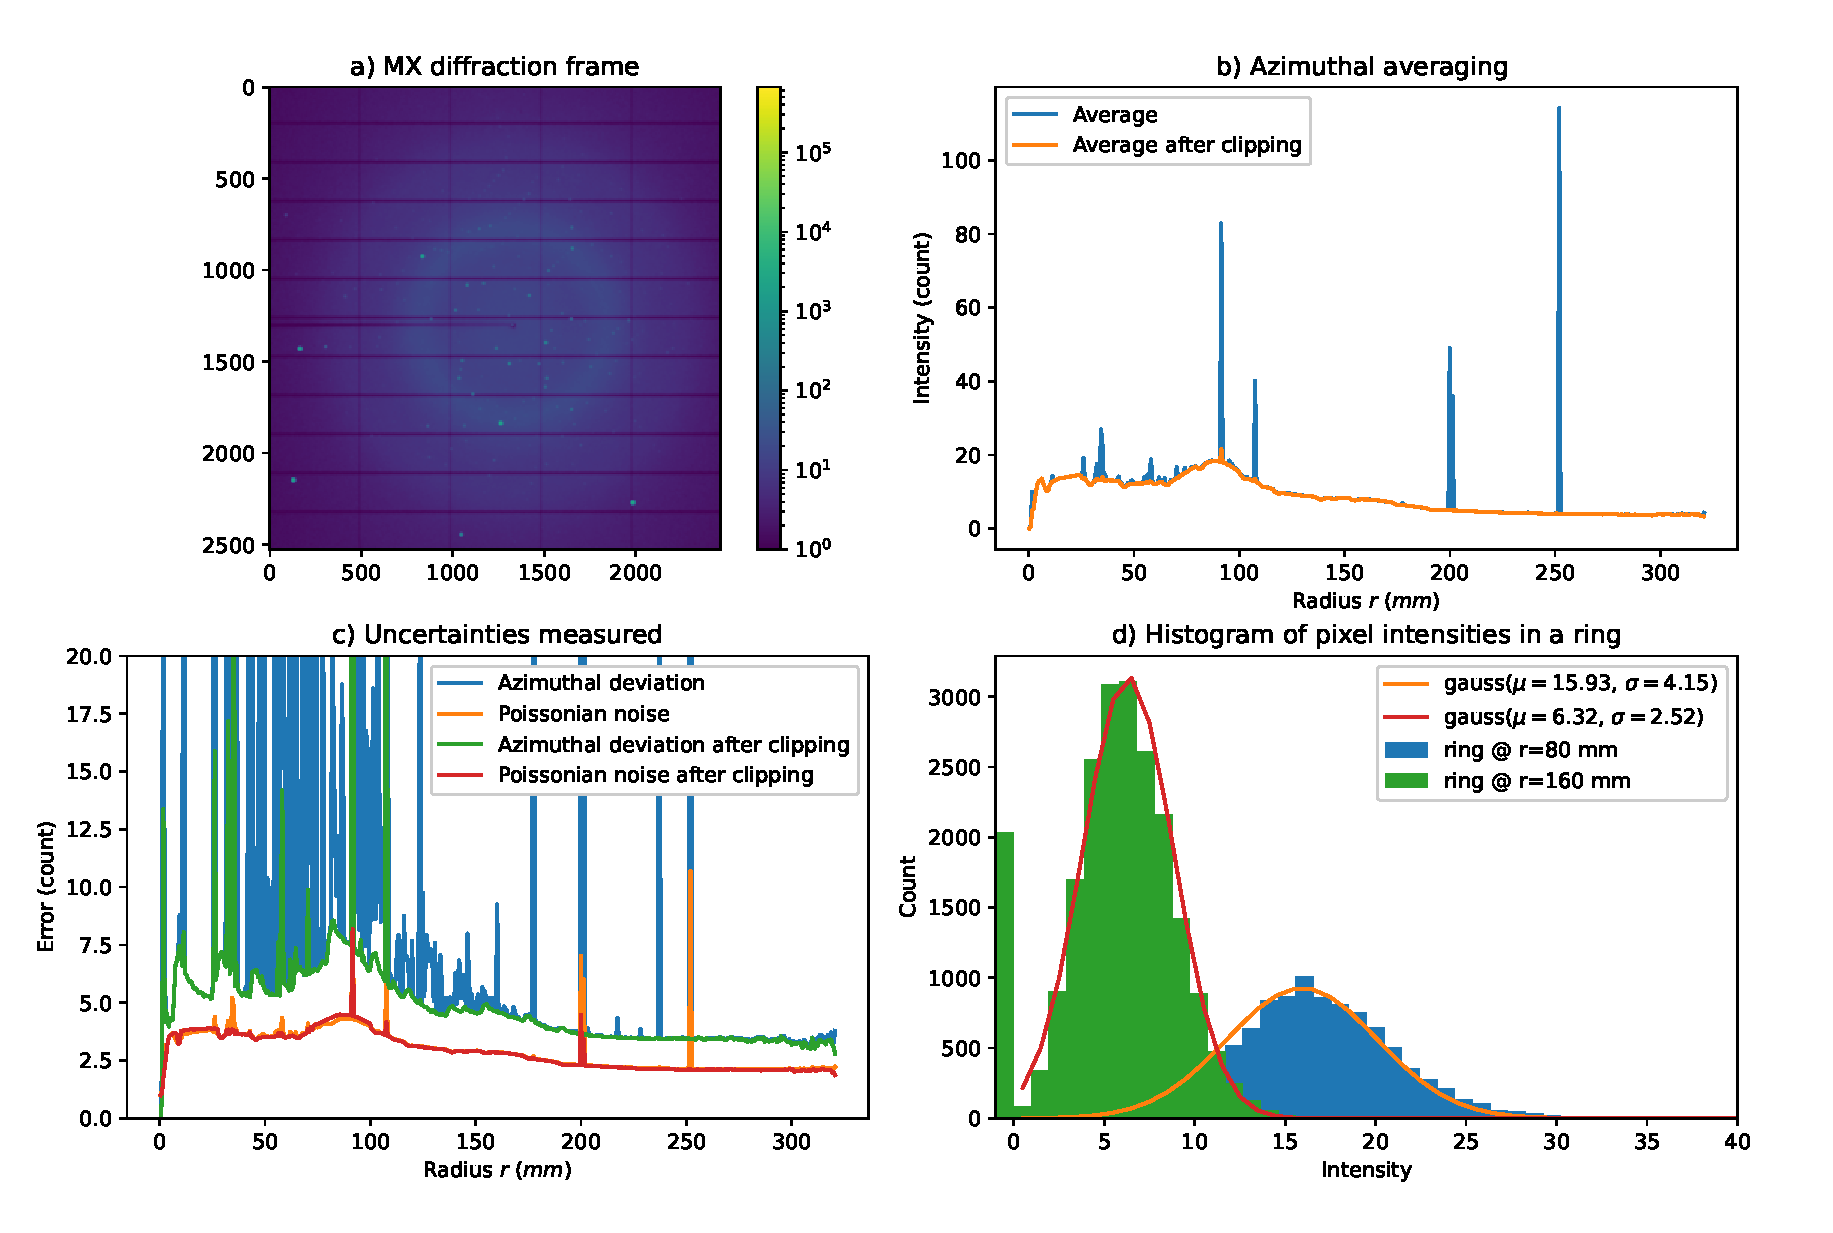
\includegraphics[width=9cm]{fig1}
\caption{Single crystal diffraction frame obtained from insulin with a Pilatus6M (a) (part of Dectris's reference dataset) with the azimuthaly averaged signal (b), 
before and after clipping data. Uncertainties are presented in (c) when calculated assuming a Poissonian error model or when measuring the deviation within all pixels in a ring.
Subplot (d) presents the histogram of intensities for two rings at r=80mm and r=160mm from beam center with the distribution fitted as gaussians.}
\end{center}
\end{figure}

The core idea of this algorithm is to model the distribution of background pixels and flag outliers like one would do in Bayesian statistical analysis \cite{Sivia2006}. 
Positive outliers can be assigned to Bragg peaks and negative outliers indicate shadows or defective pixels. 
The distribution can be re-centered on the background by discarding all pixels which intensity differ from the average value by more than $n$ times the standard deviation.
By clipping values (rejecting outliers) one enforces a gaussian distibution of the remaining values.
The orange plot in figure \ref{fig1}b presents the average after having discarded those outliers, and the orange and green curve of figure \ref{fig1}c is are the uncertainties 
calculated after this clipping. 
 After clipping the average and uncertainties curves have lost most of their spikes, which means that Bragg peaks and shadowed pixel were discarded.
 
\subsection{Sigma-clipping}
The \textit{sigma-clipping} algorithm consists in iteratively applying the outlier rejection previously described and thus enforces 
the background distribution to follow a normal law.
There are two parameters to this algorithm: the number of iterations of clipping and the rejection cut-off.

\subsubsection{Number of iterations:}
Despite the execution time is proportionnal to the number of iteration of sigma-clipping, iterations should continue until no more outliers are found and the 
background distribution actually matches a gaussian distribution. 
Since the loop exits as soon as no more outliers were discarded at the clipping step, having an arbitrary large number of iteration is not an issue for the execution time.       

\subsubsection{Clipping threshold:}
This threshold can be automatically calculated based on a variation on Chauvenet's criterion \cite{chauvenet} where one would accept to discard only one pixel in a ring with pure
background signal already following a normal law. 
Thus the threshold is adapted to the $size$ of the distribution, i.e. the number of pixels in each ring (Eq 13), which can reach several thousands and shrinks with iterations.
Typically the numerical value for this cut-off varies from 2 to 4.   
\begin{equation}
SNR_{chauvenet} =  \sqrt{2 log(\frac{size}{\sqrt{2 \pi}})}
\end{equation}

\section{Application to single crystal diffraction image compression}
Single crystal diffraction images exhibit usually an isotropic background ontop of which are Bragg peaks.
The sigma-clipping algorithm can be used to   

\section{Application to serial crystallography}

\subsection{Performance}
     % comparison with cheetah
\section{Conclusion}
drawback: textured background

     %-------------------------------------------------------------------------
     % The back matter of the paper - acknowledgements and references
     %-------------------------------------------------------------------------

     % Acknowledgements come after the appendices

\ack{Acknowledgements}



\bibliographystyle{iucr}
\bibliography{biblio}

\end{document}                    % DO NOT DELETE THIS LINE
%%%%%%%%%%%%%%%%%%%%%%%%%%%%%%%%%%%%%%%%%%%%%%%%%%%%%%%%%%%%%%%%%%%%%%%%%%%%%%
